\documentclass{article}
\usepackage[margin=0.5in]{geometry}
\usepackage{hyperref}
\usepackage{amsmath}
\usepackage{amsfonts}
\usepackage{tikz}
\usepackage{graphicx}
\usetikzlibrary{automata,positioning}
\title{Dynamic Branch Prediction Using Perceptrons}
\author{Andrew Bruce \\ \href{mailto:acbruce@ucsc.edu}{acbruce@ucsc.edu}
  \and Gowrav BG \\ \href{mailto:gbukkapa@ucsc.edu}{gbukkapa@ucsc.edu} }

\begin{document}
\maketitle
\pagenumbering{gobble}
\section*{Goal}
We aim to implement a dynamic branch predictor that uses a perceptron to adapt its weights at runtime using the perceptron training algorithm based off the 2 bit prediction history register \cite{article}.
\section*{Implementation}
We would need to create a custom branch predictor using the \verb=Bp_struct=. The history register is already handled, and we would need to use it as a ``two-level adaptive predictor'', and keep track of the counter for each of the possible 4 histories. The perceptron would then take the counters in each history of the table as counters.\\
In theory each branch would need its own perceptron, but in practice we would just index a table of perceptrons based off a hash of the branch address.\\
Each perceptron would need four weights, one for each of the histories. The global history is already implemented in scarab, so we would just need to implement the required functions for the custom branch predictor.
\begin{center}
  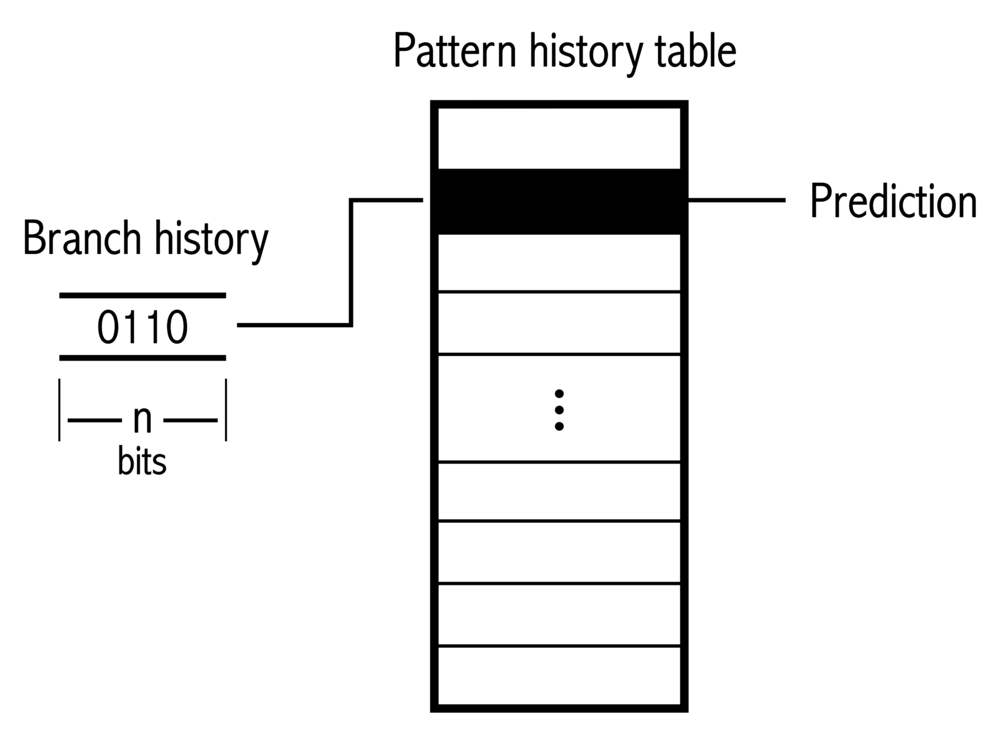
\includegraphics[width=0.3\textwidth]{table.png}
\end{center}
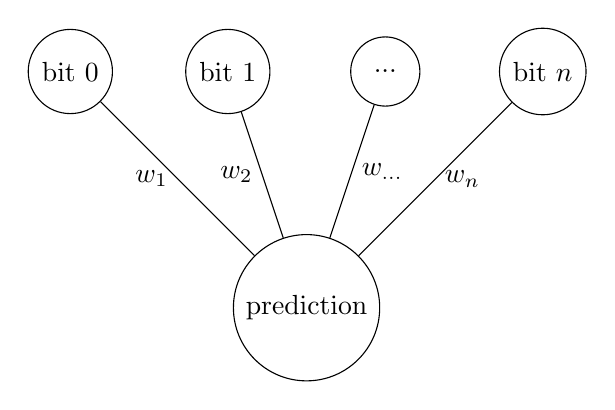
\begin{tikzpicture}
  \node[state] (q1) at (0,3) {bit 0};
  \node[state] (q2) at (2,3) {bit 1};
  \node[state] (q3) at (4,3) {...};
  \node[state] (q4) at (6,3) {bit $n$};
  \node[state] (q5) at (3, 0) {prediction};
  \draw (q1) edge [left=10pt] node {$w_1$} (q5)
        (q2) edge [left=10pt] node {$w_2$} (q5)
        (q3) edge [right=10pt] node {$w_{...}$} (q5)
        (q4) edge [right=10pt] node {$w_n$} (q5)
  ;
\end{tikzpicture}
\bibliographystyle{abbrv}
\bibliography{refs}
\end{document}
